\section{Data Transfer}

The system relies on wireless data transfer to send traffic data recorded by a camera node back to the central database. It is also useful to be able to transmit a live video feed from each node to the graphical interface so that a user may observe what the node sees in real time. Presently data transfer occurs only on a local area network. Making the network wireless was an important consideration as it allows for flexible and lightweight node installation, this was easily facilitated by the network capabilities of the Raspberry Pi. Figure \ref{fig:network_diagram} provides a high level outline of the relationships between the entities in the network.

\subsection{Video Feed}

The video feed is shared with the user interface via a simple Flask \cite{flask} application that's only functionality is uploading new images to a URL on the local network, the URL is simply embedded in the user interface as an image. Flask is a lightweight web framework for custom web services which made it optimal for the specific and small task of streaming images from a Raspberry Pi on a local network.


\subsection{Traffic Statistics}

Traffic statistics are sent to the database every 30 seconds. Simple functions implementing the MySQLConnector class \cite{mysqlconnector}\cite{mysqltutorial} were used to interface with the detection algorithm running on a camera node to the database on another machine. This connection employs transfer control protocol (TCP) which is well suited for sending small packets of data such as the traffic data though it's not as well suited to transmitting high frame rate images and so some lag can occur. 

\begin{figure}[H]
    \centering
    \centering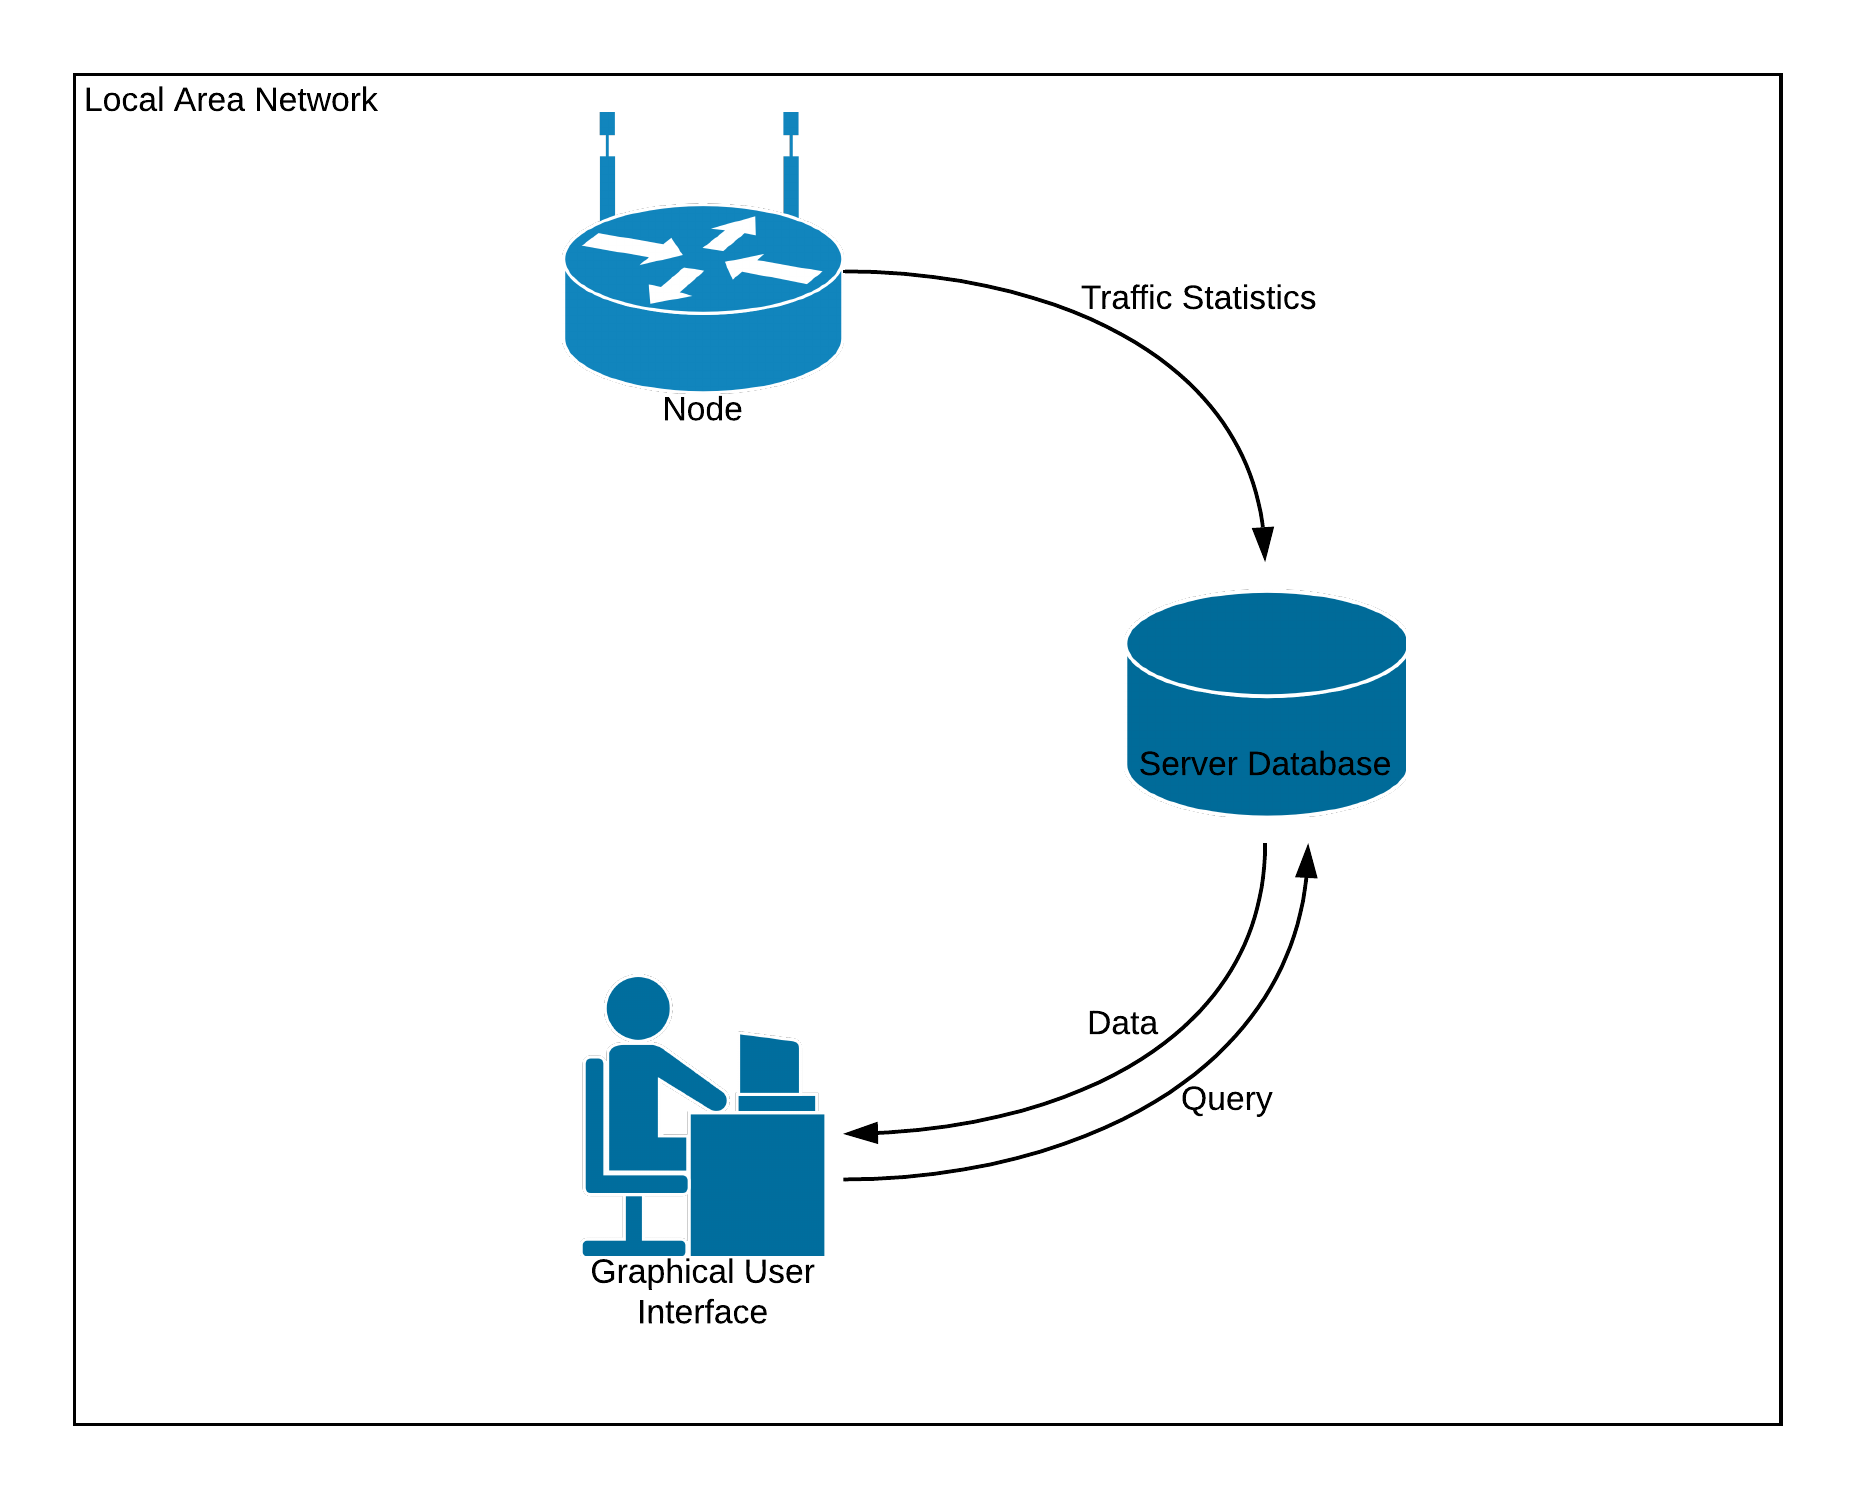
\includegraphics[width = 0.8\textwidth]{design/networking/network_diagram}
    \caption{High level operation of system network.}
    \label{fig:network_diagram}
\end{figure}